\documentclass[11pt]{article}
% Shared preamble
\usepackage[papersize={8.5in,11in},textwidth=437pt,textheight=634pt,hcentering,top=81pt,headsep=22pt,headheight=16pt]{geometry}
\usepackage[T1]{fontenc}
\usepackage{lmodern}
\usepackage{mathtools,amssymb,amsthm}
\usepackage{microtype}
\usepackage{booktabs,array}
\usepackage[font=small,labelfont=bf,labelsep=period]{caption}
\usepackage[shortlabels]{enumitem}
\usepackage{needspace}
\usepackage{tikz}
\usetikzlibrary{calc,positioning,arrows.meta}
\definecolor{ink}{HTML}{213650}
\definecolor{sea}{HTML}{19706F}
\definecolor{rust}{HTML}{AA5034}
\usepackage[numbers,sort&compress]{natbib}
\renewcommand\bibfont{\small}
\usepackage[nottoc,notlof,notlot]{tocbibind}
\usepackage{fancyhdr}
\usepackage{url}
\usepackage[colorlinks,linkcolor=ink,citecolor=sea,urlcolor=ink,psdextra]{hyperref}
\usepackage{bookmark}

\fancyhf{}
\newcommand\shorttitle{OpenAI}
\fancyhead[L]{\small\scshape\shorttitle}
\fancyhead[R]{\small\thepage}
\renewcommand\headrulewidth{0pt}
\pagestyle{fancy}
\newcommand{\articletitle}[2]{\title{\fontsize{20}{24}\selectfont\bfseries\color{ink}#1}\renewcommand\shorttitle{#2}%
  \hypersetup{pdftitle={#1},pdfauthor={OpenAI}}}
\author{OpenAI}
\date{November 24, 2026}
\setcounter{tocdepth}{1}

\newtheorem{theorem}{Theorem}[section]
\newtheorem{lemma}[theorem]{Lemma}
\newtheorem{claim}[theorem]{Claim}
\newtheorem{corollary}[theorem]{Corollary}
\newtheorem{proposition}[theorem]{Proposition}
\theoremstyle{definition}
\newtheorem{definition}[theorem]{Definition}
\newtheorem{remark}[theorem]{Remark}
\newtheorem{example}[theorem]{Example}
\numberwithin{equation}{section}
\emergencystretch=1em
\clubpenalty=3500
\widowpenalty=3500
\raggedbottom

% For numbers of results in companion papers
\makeatletter
\newcommand\ext[2]{\@ifundefined{ref@#1:#2}{??\@latex@warning{Undefined companion label #1:#2}}{\csname ref@#1:#2\endcsname}}
\newcommand\extdef[3]{\@namedef{ref@#1:#2}{#3}}
\makeatother
\extdef{G}{lem:spectral-closure}{2.1}
\extdef{G}{sec:spectra}{2}
\extdef{G}{thm:main}{1.1}


\newcommand\titlebreak{\texorpdfstring{\\}{}}
\settocbibname{References}

% Lightweight contents, with numbered bookmarks
\bookmarksetup{numbered}
\makeatletter
\renewcommand\@pnumwidth{2.1em}
\renewcommand\@dotsep{12}
\renewcommand*\l@section[2]{\addvspace{.85em}\@dottedtocline{1}{\z@}{2em}{#1\nobreak\hspace{.5em}}{#2}}
\makeatother

\articletitle{Paths, trees and grids \titlebreak separate Valiant's hierarchy}{Paths, trees and grids}
\hypersetup{pdfsubject={Paths-trees-and-grids-separate-Valiants-hierarchy-November-24-2026}}

\newcommand\VF{\mathsf{VF}_F}
\newcommand\VBP{\mathsf{VBP}_F}
\newcommand\VP{\mathsf{VP}_F}
\newcommand\VNP{\mathsf{VNP}_F}

\begin{document}
\maketitle

\begin{abstract}
We prove that \(\mathsf{VP}\ne\mathsf{VNP}\) over every field. Our
witness is the state sum on an \(n\times n\) square grid. It belongs
to \(\mathsf{VNP}\) and requires arithmetic circuits of size
\(n^{\Omega((\log n)^{1/12})}\). On binary trees and paths, the same
construction separates arithmetic circuits from algebraic branching
programs and branching programs from formulas, respectively. All
three lower bounds hold in degree-component border complexity. We
also characterize the graph families whose state sums have polynomial
size in each model.
\end{abstract}

\section{Introduction}\label{sec:introduction}

An exponentially long sum can have a short arithmetic computation.
Choose one variable from each of the \(n\) pairs \((x_i,y_i)\) and
multiply the chosen variables. There are \(2^n\) choices. Their
products sum to \(\prod_{i=1}^n(x_i+y_i)\).
Now suppose a polynomial-size arithmetic circuit takes a string of
polynomially many bits as an additional input and computes the term
indexed by that string. Can the sum over all strings always be
computed by a polynomial-size circuit? Valiant's class
\(\mathsf{VNP}\) allows this summation~\cite{Valiant}. Membership in
\(\mathsf{VP}\) requires a polynomial-size circuit for the resulting
polynomial itself. We prove that \(\mathsf{VP}\ne\mathsf{VNP}\) over
every field.

Our witness is a polynomial on a square grid. Give each edge a label
and place a table of independent variables at each vertex. A labeling
of the grid selects one entry at each vertex according to the labels
on the edges meeting there. The product of those entries is the
weight of the labeling. On an \(n\times n\) grid with \(n\) possible
labels per edge, a polynomial-size circuit can compute this weight
from the labels. Summing the weights over all labelings gives the
grid's \emph{state sum}. We show that its circuit size grows
superpolynomially with \(n\), even allowing cancellations and
unrestricted reuse of intermediate values.

The same construction on two simpler graphs separates the models
within \(\mathsf{VP}\). On a complete binary tree, a polynomial-size
circuit can compute and reuse the contributions from its subtrees.
Algebraic branching programs (ABPs) require superpolynomial size for
this family. On a path, the state sum is an entry of a product of
matrices. A branching program can evaluate it by remembering the
state of the current edge, and here the superpolynomial lower bound
is for arithmetic formulas. Over a field \(F\), we write \(\VF\)
and \(\VBP\) for the polynomial-size formula and branching-program
classes. In all four classes the number of variables and the output
degree are polynomially bounded in the family index.

\needspace{15\baselineskip}
\begin{theorem}[Three separations]\label{thm:main}
Over every field \(F\),
\[
             \VF\subsetneq\VBP\subsetneq\VP\subsetneq\VNP .
\]
With \(n\) states per edge, the following graph families witness the
three strict inclusions. The lower bounds hold in degree-component
border complexity, with absolute constants for all sufficiently large \(n\).
\begin{center}
\small\normalfont
\begin{tabular}{@{}ll@{\hspace{1.15em}}l@{}}
\toprule
Graph & Upper class & Lower bound \\
\midrule
\(n\times n\) square grid & \(\VNP\) & Circuit size \(n^{\Omega((\log n)^{1/12})}\)\\
Complete binary tree, \(\lfloor\log_2(2n)\rfloor\) levels &
\(\VP\) & ABP size \(n^{\Omega(\sqrt{\log\log n})}\)\\
Path on \(n\) vertices & \(\VBP\) & Formula size \(n^{\Omega(\log\log n)}\)\\
\bottomrule
\end{tabular}
\end{center}
The determinant of an \(n\times n\) matrix of independent variables also
has degree-component border formula size at least \(n^{\Omega(\log\log n)}\).
\end{theorem}

To write the state sum explicitly, let \(G=(V,E)\) be a finite loopless multigraph
and let \(E(v)\) be the list of edges at \(v\). For each assignment
\(\alpha\in[q]^{E(v)}\), where \([q]=\{1,\ldots,q\}\), let
\(X_{v,\alpha}\) be the corresponding table entry. With \(q\) states
per edge, the polynomial is
\begin{equation}\label{eq:graph}
       Z_{G,q}(X)=\sum_{a\in[q]^E}\prod_{v\in V}X_{v,a|_{E(v)}} .
\end{equation}
For the grid, the \(\VNP\) description works in every characteristic.
A binary string encodes the labels. Boolean indicators pick out the
corresponding table entry at each vertex, and unused encodings
contribute zero. Since at most four edges meet at a vertex, there are
at most \(n^4\) entries to choose from in each table. The circuit lower
bound allows arbitrary constants, affine inputs, and limits over the
algebraic closure of \(F\) after taking the component of the required
degree (Section~\ref{sec:notation}).

For the three-vertex path, Equation~\eqref{eq:graph} is
\(\sum_{i,j=1}^q x_iY_{ij}z_j\), the product of a row, a matrix and a
column. The formula bound is sharp in a regime that already suffices to
separate \(\VF\) from \(\VBP\). For a path on \(d\) vertices with \(q\)
states on each edge, bisection gives a formula of size \(q^{O(\log d)}\).
Theorem~\ref{thm:full-flat-graph} gives the matching
\(q^{\Omega(\log d)}\) bound for \(2\le d\le(\log q)^{1/3}\), and its
lower bound holds for every tree of that order. A short path already
suffices for the determinant bound in Theorem~\ref{thm:main}, because
its polynomial is a signed cofactor of a polynomial-size matrix of
affine forms.

For arbitrary graph families, these witnesses give a classification.
Consider a single polynomial bound on the size of \(Z_{G,q}\) in
\(|V(G)|+q\), uniformly over the family and all \(q\ge2\).
Formulas admit such a bound exactly when both the maximum degree and
the order of the largest connected component are bounded. For ABPs the
criterion is bounded cutwidth. For circuits it is bounded treewidth
and bounded maximum degree. Large graphs violating these conditions
either have a large table at one vertex or contain the corresponding
witnesses as minors (Theorem~\ref{thm:graph-classification}).

\needspace{7\baselineskip}
\subsection*{How the three lower bounds fit together}

The coefficients of \(Z_{G,q}\) record one constraint per edge. A
monomial selects one table entry at every vertex, and its coefficient
is one precisely when the entries agree on the state at both ends of
every edge. Thus the coefficient tensor consists of independent
equality constraints. The Euclidean price theorem of the first
paper~\cite{oaG}, based on Strassen's asymptotic spectrum~\cite{Strassen},
assigns a cost to sharing a label at chosen sites in Euclidean space.
We place the two ends of each edge at opposite unit vectors on an axis
of its own. The cost of
the graph tensor at these terminals is then the sum of the individual
edge costs.

A small computation expresses the coefficient tensor as a sum of terms
with simpler dependencies. Suppose a term has matrix rank \(R\) across
a cut separating the vertex tables into two groups. Its rank
factorization can be supplied by sharing a single \(R\)-valued label
between two auxiliary sites. For each term we may choose those sites
to suit its cut while delivering each edge-end index to its assigned
terminal. That terminal stays fixed across all summands. Moving one
supply site to shorten the total length of its output wires yields a
saving governed by the number of crossing edges. If \(R\)
is small and sufficiently many edges cross, the term costs less than
the graph tensor. A single Euclidean price bounds the sum, including
when the low-rank cut differs from term to term
(Section~\ref{sec:cuts}).

\begin{figure}[!hbp]
\centering
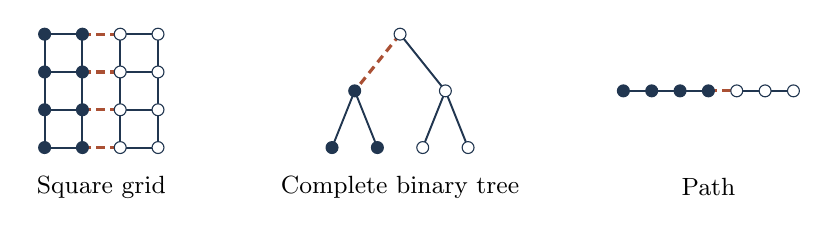
\begin{tikzpicture}[x=.48cm,y=.48cm,font=\small,
 ordinary/.style={draw=ink,line width=.7pt},
 crossing/.style={draw=rust,densely dashed,line width=1.15pt},
 chosen/.style={circle,draw=ink,fill=ink,inner sep=0pt,minimum size=4.3pt},
 outside/.style={circle,draw=ink,fill=white,inner sep=0pt,minimum size=4.3pt}]
\begin{scope}
  \foreach \i in {0,...,3} {
    \draw[ordinary] (\i,0)--(\i,3);
    \draw[ordinary] (0,\i)--(1,\i) (2,\i)--(3,\i);
    \draw[crossing] (1,\i)--(2,\i);
  }
  \foreach \i in {0,...,3} {
    \foreach \j in {0,1} \node[chosen] at (\j,\i) {};
    \foreach \j in {2,3} \node[outside] at (\j,\i) {};
  }
  \node at (1.5,-1.05) {Square grid};
\end{scope}
\begin{scope}[xshift=3.65cm]
  \coordinate (root) at (1.8,3);
  \coordinate (l) at (.6,1.5); \coordinate (r) at (3,1.5);
  \coordinate (ll) at (0,0); \coordinate (lr) at (1.2,0);
  \coordinate (rl) at (2.4,0); \coordinate (rr) at (3.6,0);
  \draw[crossing] (root)--(l);
  \draw[ordinary] (root)--(r) (l)--(ll) (l)--(lr) (r)--(rl) (r)--(rr);
  \foreach \v in {l,ll,lr} \node[chosen] at (\v) {};
  \foreach \v in {root,r,rl,rr} \node[outside] at (\v) {};
  \node at (1.8,-1.05) {Complete binary tree};
\end{scope}
\begin{scope}[xshift=7.35cm]
  \draw[ordinary] (0,1.5)--(2.25,1.5) (3,1.5)--(4.5,1.5);
  \draw[crossing] (2.25,1.5)--(3,1.5);
  \foreach \i in {0,...,3} \node[chosen] at (.75*\i,1.5) {};
  \foreach \i in {4,...,6} \node[outside] at (.75*\i,1.5) {};
  \node at (2.25,-1.05) {Path};
\end{scope}
\end{tikzpicture}
\caption{Three cuts between filled and open vertices. Four edges
cross the middle of this grid. On the binary tree a balanced split
can cross just one edge, so the ABP argument prescribes the size of
the smaller set more carefully. On the path, a proper nonempty prefix
of any size cuts just one edge. The formula argument combines splits
at several scales.}
\label{fig:witness-cuts}
\end{figure}


Figure~\ref{fig:witness-cuts} illustrates why the proofs proceed from
grids to trees to paths. Each model controls a different set of cuts.
\begin{itemize}[leftmargin=*,itemsep=.35ex]
\item \emph{Grids.} In a small circuit, decomposing at gates of
intermediate degree gives one low-rank cut per summand. Both sides
contain at least a third of the vertices. Every such cut of an
\(r\times r\) grid crosses \(\Omega(r)\) edges
(Section~\ref{sec:grid}).
\item \emph{Binary trees.} A tree can have a balanced cut consisting of
a single edge. An ABP gives more information. In each contributing term of the ABP path expansion, the variables
appear in some order. We can stop after any prescribed number \(k\) of
groups. There is a \(k\) for which
every \(k\)-vertex subset of the complete binary tree has many
boundary edges (Section~\ref{sec:bt}).
\item \emph{Paths.} For every nontrivial cardinality a path has a
prefix of that size with just one boundary edge. A formula, however,
splits the variable groups recursively. We choose the auxiliary
sites to charge its nested splits at several scales at once. The
mean-width formula bounds the cost of each label shared by the
leaves below a split (Section~\ref{sec:formula}).
\end{itemize}

The quantitative estimates first apply to small graphs with many states
per edge. In this regime the saving in each term exceeds the cost of
summing over terms. Projection transfers the bounds to the larger
witnesses in Theorem~\ref{thm:main}. The same transfer, now through
graph minors, gives the classification in
Section~\ref{sec:graph-classification}.

\subsection*{Relation to earlier work}

Valiant introduced $\VP$ and $\VNP$ to study efficient arithmetic
computation under polynomial projections~\cite{Valiant,Burgisser}.
The determinant is complete for $\VBP$ under such projections
\cite{Toda,MalodPortier,MahajanVinay}. Its formula complexity therefore
measures the cost of simulating branching programs by formulas.
The depth reduction of Valiant, Skyum, Berkowitz and Rackoff
\cite{VSBR} gives every family in $\VP$ formulas of
quasipolynomial size. A classical lower bound of Kalorkoti
\cite{Kalorkoti} gives $\Omega(n^3)$ for the order-$n$ determinant over
any field, counting variable and constant occurrences even in formulas
with division.

Many earlier separations use restrictions on the computation. Nisan's
coefficient matrices give exponential branching-program lower bounds
for explicit noncommutative polynomials~\cite{Nisan}. Raz proved
superpolynomial multilinear formula bounds for the determinant and
permanent, separated multilinear formulas from circuits, and related
formula size to tensor rank~\cite{RazMultilinear,RazFormula,RazRank}.
Dvir, Malod, Perifel and Yehudayoff separated multilinear formulas
from multilinear branching programs~\cite{DMPY}. For iterated matrix
multiplication itself, lower bounds are known for monotone formulas
\cite{Snir}, set-multilinear formulas~\cite{LST}, and constant-depth
circuits~\cite{LstDepth,Forbes,BDS}. The formulas and circuits of
Theorem~\ref{thm:main} may use arbitrary field constants and have
unbounded depth and nonmultilinear intermediate gates.

Graph structure also governs several related models. Hrube\v{s} and
Yehudayoff used the edge boundary of vertex sets of a prescribed size
in a binary tree to separate monotone branching programs from monotone
circuits~\cite{HrubesYehudayoff}. For graph homomorphism polynomials,
Komarath, Pandey and Rahul characterized monotone formula,
branching-program and circuit complexity by the treedepth, pathwidth
and treewidth of the pattern graph~\cite{KPR}. Homomorphism polynomials
also yield complete families for $\VP$~\cite{Durand} and separations
between symmetric models of arithmetic computation~\cite{dw,DPS}.
The classification in Theorem~\ref{thm:graph-classification} concerns
the state sum with an independent table of variables at each vertex.

For general circuits, an earlier bound for the order-$n$ permanent over
$\mathbb C$ was $\Omega(n^2\log\log n)$ with binary gates and individual
variable or scalar inputs~\cite[Chapter~5]{TenAdvances}. A companion paper~\cite{oaP} gives stronger circuit
bounds for the Hamiltonian cycle polynomial and, outside characteristic
two, the permanent. For the geometric study of determinantal
representations and their closures, see~\cite{MS}.

\section{Arithmetic models and projections}\label{sec:notation}

All polynomials are formal and commutative. A circuit over \(F\) uses
binary addition, subtraction, and multiplication gates. Its size \(s\)
counts the operation gates. A formula is a circuit with a tree of
gate occurrences. We allow an arbitrary affine form in the input
variables at each leaf, free of charge. An ABP sums products of affine edge labels along source--sink paths in
a directed acyclic graph. Its size counts both vertices and edges. These input conventions preserve the
polynomial-size classes for families of polynomially bounded arity.
We impose no bound on the degree of intermediate computations.
Throughout, logarithms have base two.

Series and parallel composition turn a formula into a branching program
of linear size. A circuit can evaluate a branching program in
topological order, summing at each vertex the value at each predecessor
times the connecting edge label. Finally, a family in \(\VNP\) has the
form
\[
          f_n(X)=\sum_{b\in\{0,1\}^{p(n)}}g_n(b,X)
\]
for a polynomially bounded \(p(n)\) and \((g_n)\in\VP\). Taking
\(p(n)=0\) gives the last inclusion in Theorem~\ref{thm:main}.

\paragraph{Degree-component border size.}
Fix a homogeneous target of degree \(D\) and put \(K=\overline F\).
The target has \emph{degree-component border size} at most \(s\) if
its coefficient vector lies in the Zariski closure, over \(K\), of the
degree-\(D\) components of outputs of size-\(s\) or smaller computations
in the specified model. Approximating outputs can have terms in other
degrees. The following lemma accounts for those terms when a substitution
uses constants and lowers the degree.

\begin{lemma}[Projection]\label{lem:projection}
Let \(f\) be homogeneous of degree \(D\) and suppose that substituting
affine forms for its variables gives a homogeneous polynomial \(g\).
If \(f\) has degree-component border size at most \(s\), then in the
same model \(g\) has degree-component border size at most
\(O((s+1)(D+1)^2)\) for circuits and \(O((s+1)^2)\) for formulas or ABPs.
\end{lemma}
\begin{proof}
First extract the degree-\(D\) component of each approximating output.
A circuit computes all components through degree \(D\) at each gate,
using convolution at multiplication gates. This uses
\(O((s+1)(D+1)^2)\) gates. A size-\(s\) formula or ABP has output degree
at most \(s+1\). Over the infinite field \(K\), interpolation in
\(t\) at \(s+2\) distinct values isolates degree \(D\) in the scaled
output \(f_{\rm out}(tX)\). If \(D>s+1\) the component is zero.
Combining the scaled copies otherwise costs \(O((s+1)^2)\).

Substitute the prescribed affine forms in the extracted component
and read its component of degree \(\deg g\). For the target this
returns \(g\). From the degree-\(D\) coefficient space to the
degree-\(\deg g\) coefficient space, the resulting map is linear.
It therefore takes the original target into the closure of the
transformed outputs, with the stated size bound.
\end{proof}

\paragraph{Subgraphs and smaller alphabets.}
The polynomial \(Z_{G,q}\) is homogeneous of degree \(|V(G)|\) and
set-multilinear in the vertex tables. For a subgraph \(H\subseteq G\)
and \(2\le q'\le q\), a substitution of variables, zero, and one sends
\(Z_{G,q}\) to \(Z_{H,q'}\). Pin each unused edge to state one and allow
only the first \(q'\) states on the retained edges. A table entry
inconsistent with these choices is set to zero. A consistent entry
becomes the corresponding variable at a retained vertex and becomes
one at a deleted vertex. Each labeling of \(H\) has exactly one
surviving extension to \(G\). This gives the projections used in the
three witness proofs. Lemma~\ref{lem:graph-minor} extends the construction
to graph minors.

\section{A common price for different cuts}\label{sec:cuts}

Write $d=|V(G)|$, $e=|E(G)|$ and $w=\log q$. The variables in the
table at a vertex $v$ form a \emph{slot}. For a polynomial $f$ in
these variables, let $A(f)$ be the array of coefficients of monomials
containing exactly one variable from each slot. An index at $v$
specifies a table entry and hence a tuple of $\deg(v)$ edge labels.
We write this tuple as $\deg(v)$ separate indices of dimension $q$,
in the table basis. An isolated vertex contributes a one-dimensional
factor.

For the graph polynomial $Z_{G,q}$, a coefficient is one precisely when
the two endpoint labels agree on every edge. Thus $A(Z_{G,q})$ is a
tensor product, with one equality wire $\sum_{i=1}^q e_i\otimes e_i$
per edge. Across a fixed bipartition $C\mid V(G)\setminus C$ of the
slots its matrix rank is $q^{|\partial C|}$, where $\partial C$ is the
set of edges crossing the cut. Each crossing wire is an identity matrix
of rank $q$, and each internal wire is a nonzero vector on one side.
In the circuit and branching-program decompositions below, different
summands can have low rank across different cuts. We will use a
single tensor invariant that detects a saving on each summand and
controls the price of their sum.

\subsection*{Euclidean tensor prices}

We use the following consequences of the Euclidean price theorem
\cite[Theorem~\ext{G}{thm:main}, Section~\ext{G}{sec:spectra} and
Lemma~\ext{G}{lem:spectral-closure}]{oaG}. We work over the algebraic
closure $K=\overline F$ so that the same comparison applies to border
computations.

\begin{theorem}[Euclidean pricing]\label{thm:width}
Fix a Euclidean space of any finite dimension. Assign every index of a
finite tensor over $K$ to a site in this space, grouping all indices at
one site into a single factor. There is one compatible system of prices
$H(T)$ for all such placements. Adjoining an unused site leaves the
price unchanged. The price is real for $T\ne0$, and $H(0)=-\infty$.
\begin{enumerate}[leftmargin=*,itemsep=.3ex]
\item Tensor products add prices. Applying one linear map to the entire
factor at each site cannot increase the price.
\item Sharing a common $q$-valued label among a finite nonempty set $S$
of sites costs $\delta(S)\log q$, where
\[
       \delta(S)=\sqrt{2\pi}\,\mathbb E\max_{x\in S}\langle g,x\rangle
\]
for a standard Gaussian vector $g$. This is the Gaussian mean width
of the convex hull, normalized to give a segment its length. In particular, $\delta(\{x,y\})$
is the distance between $x$ and $y$.
\item For tensors in the same format placed at the same sites $S$,
their ordinary sum satisfies
\begin{equation}\label{eq:ordinary}
 H(T_1+\cdots+T_L)\le \max_{1\le i\le L} H(T_i)+\delta(S)\log L .
\end{equation}
\item In each fixed format and placement, the price sublevels
$\{T:H(T)\le a\}$ are Zariski closed.
\end{enumerate}
\end{theorem}

An arbitrary array on indices at a single site can be supplied by a
local linear map from a scalar. To deliver an index of dimension $q$
from that site to a site at distance $D$, contract it with one end of an
equality wire and use the other end as the output index. The wire costs
$Dw$. We can choose the auxiliary sites for this construction separately
for each summand. Only the common \emph{output} sites enter the sum
penalty in Equation~\eqref{eq:ordinary}.

For any finite nonempty set $S$ in the unit ball we have
\begin{equation}\label{eq:width-ball}
                         \delta(S)=O\bigl(\sqrt{\log(2|S|)}\bigr).
\end{equation}
Indeed each $\langle g,x\rangle$ has variance at most one. A union bound
gives $\Pr(\max_{x\in S}\langle g,x\rangle>t)\le |S|\exp(-t^2/2)$ for
$t\ge0$, and integration of the tail gives the stated estimate.

\subsection*{Fixed terminals and movable supply sites}

Give each edge its own coordinate axis in $\mathbb R^e$. Place its
two endpoint indices at the opposite unit vectors on that axis, choosing
the signs arbitrarily. Call these $2e$ sites the \emph{terminals}.
The target price at the terminals is
\[
                          H(A(Z_{G,q}))=2ew ,
\]
since each of its $e$ wires has length two. We could supply any tensor
of this format by putting its whole array at the origin and sending
each of its $2e$ indices one unit to its terminal. The graph tensor
attains this upper bound. To prove a lower bound, we will exploit a
summand's cut to supply it for strictly less.

Let $a_v$ be the sum of the terminal vectors of slot $v$. For
$C\subseteq V(G)$ set $a_C=\sum_{v\in C}a_v$. The two endpoints of
each edge internal to $C$ cancel, and the edges leaving $C$ contribute
one unit vector each on mutually orthogonal axes. Consequently
\begin{equation}\label{eq:cut}
                       \|a_C\|^2=|\partial C|.
\end{equation}
If the slots in $C$ are supplied at $z$ instead of the origin, the
distance to a unit terminal $u$ changes by at most
$-\langle z,u\rangle+\|z\|^2/2$, since
$\sqrt{1-2\langle z,u\rangle+\|z\|^2}
 \le 1-\langle z,u\rangle+\|z\|^2/2$. The change in the total
distance to the terminals belonging to $C$ is therefore at most
\begin{equation}\label{eq:move}
                -\langle z,a_C\rangle+
                    \tfrac12\|z\|^2\sum_{v\in C}\deg(v).
\end{equation}
Moving a short distance in the direction of $a_C$ saves wire length at
first-order rate $\sqrt{|\partial C|}$. The following estimate
compares that saving with the cost of sharing a rank label across the
cut, as illustrated in Figure~\ref{fig:move}.
\begin{figure}[htbp]
\centering
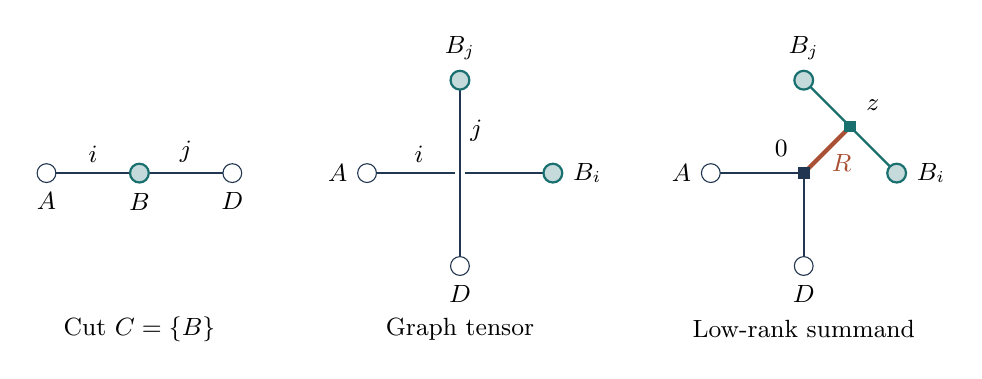
\begin{tikzpicture}[x=1.18cm,y=1.18cm,font=\small,
  t/.style={circle,draw=ink,fill=white,inner sep=2.4pt},
  c/.style={t,draw=sea,fill=sea!25,thick},
  wire/.style={draw=ink,thick}, cutwire/.style={draw=sea,thick},
  supply/.style={rectangle,fill=ink,inner sep=2.1pt}]
\begin{scope}[shift={(-3.45,0)}]
  \draw[wire] (-1,0)--node[midway,above]{$i$}(0,0)--node[midway,above]{$j$}(1,0);
  \node[t,label=below:$A$] at (-1,0) {};
  \node[c,label=below:$B$] at (0,0) {};
  \node[t,label=below:$D$] at (1,0) {};
  \node at (0,-1.68) {Cut $C=\{B\}$};
\end{scope}
\begin{scope}
  \draw[wire] (-1,0)--node[pos=.28,above]{$i$}(1,0);
  \draw[wire,preaction={draw=white,line width=3.8pt}] (0,-1)--node[pos=.73,right]{$j$}(0,1);
  \node[t,label=left:$A$] at (-1,0) {};
  \node[c,label=right:$B_i$] at (1,0) {};
  \node[c,label=above:$B_j$] at (0,1) {};
  \node[t,label=below:$D$] at (0,-1) {};
  \node at (0,-1.68) {Graph tensor};
\end{scope}
\begin{scope}[shift={(3.7,0)}]
  \coordinate (o) at (0,0);
  \coordinate (z) at (.5,.5);
  \draw[wire] (-1,0)--(o)--(0,-1);
  \draw[cutwire] (1,0)--(z)--(0,1);
  \draw[rust,line width=1.5pt] (o)--node[midway,below right,inner sep=1pt]{$R$}(z);
  \node[supply,label=above left:$0$] at (o) {};
  \node[supply,fill=sea,label=above right:$z$] at (z) {};
  \node[t,label=left:$A$] at (-1,0) {};
  \node[c,label=right:$B_i$] at (1,0) {};
  \node[c,label=above:$B_j$] at (0,1) {};
  \node[t,label=below:$D$] at (0,-1) {};
  \node at (0,-1.68) {Low-rank summand};
\end{scope}
\end{tikzpicture}
\caption{On the path $A$--$B$--$D$, the indices $i$ and $j$ of slot
$B$ occupy separate terminals $B_i$ and $B_j$. Each edge of the graph
gives a length-two equality wire between opposite terminals, for a
total price of $4w$. For a summand of rank at most $R$ across
$\{B\}\mid\{A,D\}$, the squares mark the two supply sites. Moving the
site $z$ toward both terminals of $B$ shortens their $q$-dimensional
wires. The wire from $0$ to $z$ has dimension $R$ and costs
$\|z\|\log R$.}\label{fig:move}
\end{figure}


\begin{lemma}[One cut per summand]\label{lem:single}
Let $G$ have $d$ vertices and $e$ edges, with
$2\le d\le w^{1/3}$, $1\le e\le 2d$ and $w=\log q$.
Fix $1\le b\le e$. Suppose $A(Z_{G,q})$ lies in the Zariski closure
of sums of at most $2^d$ tensors with the following property. For each
summand there is a bipartition of slots $C\mid V(G)\setminus C$ with
$|\partial C|\ge b$ across which that summand has matrix rank at most
$R$. Then for all sufficiently large $w$,
\[
                             \log R\ge \tfrac12 w\sqrt b .
\]
\end{lemma}

\begin{proof}
Suppose $\log R< w\sqrt b/2$, and fix one summand $T$ with its cut
$C$. A rank factorization across $C$ writes
$T=\sum_{i=1}^R U_i\otimes V_i$, with $U_i$ on the slots in $C$ and
$V_i$ on the remaining slots. Put the two supply sites at
$z=\lambda a_C/\|a_C\|$ and $0$. A single $R$-dimensional equality
wire between them supplies the common index $i$. The local maps
$e_i\mapsto U_i$ and $e_i\mapsto V_i$ produce the two sets of indices,
which are then sent to their fixed terminals. The rank wire costs
$\lambda\log R$. By Equations~\eqref{eq:cut} and~\eqref{eq:move},
the wires to the terminals save at least $\lambda w\sqrt b-ew\lambda^2$
against the original budget of $2ew$. Taking $\lambda=\sqrt b/(4e)$
gives
\[
 H(T)\le 2ew-\lambda(w\sqrt b-\log R)+ew\lambda^2
      \le 2ew-\frac{wb}{16e}.
\]

All the summands now have prices at the same $2e$ terminals. Adding
at most $2^d$ of them costs at most $O(d\sqrt{\log(2d)})$ above their
largest price by Equations~\eqref{eq:ordinary} and~\eqref{eq:width-ball}.
This is at most $wb/(32e)$ for all sufficiently large $w$, uniformly
in the given ranges, since $e\le2d$, $b\ge1$ and $d\le w^{1/3}$.
Thus the sums and their Zariski closure lie in the sublevel
$H\le2ew-wb/(32e)$. The graph tensor has price $2ew$, a contradiction.
\end{proof}

\section{Square grids and general circuits}\label{sec:grid}

Let $G_n$ be the $n$-by-$n$ square grid. Summation over edge labels
places the family $(Z_{G_n,n})_n$ in $\VNP$. For the circuit lower
bound, we use the fact that every partition
placing at least a third of the vertices on each side cuts many edges.
A small circuit would express the coefficient tensor as a sum in which
each term has low rank across some such partition. The partition may
vary with the term, as permitted in Lemma~\ref{lem:single}.

\begin{theorem}[Grid circuit lower bound]\label{thm:grid}
Let $G$ be the $r$-by-$r$ square grid, where
$r\ge2$ and $r^2\le(\log q)^{1/3}$. Over every field, the state sum
$Z_{G,q}$ has degree-component border circuit size at least
$q^{\Omega(\sqrt r)}$ for all sufficiently large $q$.
\end{theorem}

To obtain the partitions, we decompose the degree-$d$ component of
the circuit output into products of homogeneous factors of balanced
degrees. This is a gate decomposition of the kind used by Valiant,
Skyum, Berkowitz and Rackoff~\cite{VSBR}. Extracting the coefficients with one variable per slot turns each
product into outer products across balanced sets of grid vertices.

\begin{lemma}[Balanced slot sets]\label{lem:balanced}
Suppose the variables are grouped into a set $V$ of $d\ge2$ slots, and
a commutative arithmetic circuit of size $s$ computes $f$. Its slot
tensor has a decomposition
\[
 A(f)=\sum_{\substack{U\subseteq V\\d/3<|U|\le 2d/3}}T_U ,
 \qquad
 \operatorname{rank}_{U\mid V\setminus U}(T_U)
 \le C(s+1)(d+1)^2
\]
with an absolute constant $C$. In particular there are at most $2^d$
terms. For a homogeneous target of degree $d$ and degree-component
border circuit size at most $s$, the slot tensor belongs to the
Zariski closure of the set of such sums.
\end{lemma}

\begin{proof}
Write $[f]_d$ for the degree-$d$ component of $f$. At every gate,
compute all homogeneous components through degree $d$, using
convolution at products. This gives a homogeneous circuit for $[f]_d$
with at most $C(s+1)(d+1)^2$ gates and inputs. The count includes
splitting each of the $O(s+1)$ affine inputs used by the original
circuit into its constant and linear parts.

We maintain an expression for $[f]_d$ as a sum of products $Q_vP_v$,
where $P_v$ is the polynomial at gate $v$ and $Q_v$ is its multiplier.
Initially the only term is the output, with multiplier one. Process
gates in reverse topological order, adding all multipliers at each gate
before processing it. Retain a term when $\deg P_v\le 2d/3$. At a
sum or difference of higher degree, distribute $Q_v$ to both inputs
with the appropriate signs. At a product $P_v=P_uP_t$, choose an
input of larger degree, say $u$, and pass the multiplier $Q_vP_t$ to
$u$. In a tie choose the first input position. This identity works
also for a square in characteristic two. Throughout, take gate degrees
from the homogeneous construction and omit zero terms.

Each step preserves the polynomial represented by the sum. A sum gate
preserves degree along each input, and the larger input of a product
of degree greater than $2d/3$ has degree greater than $d/3$.
Consequently the retained terms give an identity
\[
 [f]_d=\sum_v Q_vP_v,\qquad d/3<\deg P_v\le 2d/3,\qquad
 \deg Q_v=d-\deg P_v .
\]
The number of terms is at most the number of gates and inputs in the
homogeneous circuit, since each retained gate has a single accumulated
multiplier.

For $U\subseteq V$ let $A_U(P)$ denote the array of coefficients of
monomials in $P$ containing one variable from each slot of $U$ and
no other variables. In any contribution to a slot coefficient of
$Q_vP_v$, the variables contributed by $P_v$ occupy some set $U$ of
size $\deg P_v$. The variables contributed by $Q_v$ occupy its
complement. Collecting contributions for each $U$ gives
\[
 T_U=\sum_{v:\,\deg P_v=|U|}
       A_U(P_v)\otimes A_{V\setminus U}(Q_v),
\]
where the tensor factors are placed in the original slot order. Each
summand has rank at most one across this cut, which gives the asserted
rank bound. Finally, $A(f)=A([f]_d)$, and the coefficient map on the
space of homogeneous degree-$d$ polynomials is linear. It therefore
takes the closure defining border size into the closure of the sums
above.
\end{proof}

\begin{proof}[Proof of Theorem~\ref{thm:grid}]
Put $d=r^2$. Color the vertices according to the two sides of a cut in
Lemma~\ref{lem:balanced}. Each color occupies at least $r^2/3$
vertices. If at least $r/3$ rows contain both colors, each of these
rows supplies a horizontal crossing edge. Otherwise the mixed rows
contain fewer than $r^2/3$ vertices altogether. Each color must then
occupy an entire row, so every column supplies a vertical crossing
edge. In both cases the boundary has size at least $\lceil r/3\rceil$.

Let $s$ be the degree-component border circuit size of $Z_{G,q}$.
The grid has $e=2r(r-1)\le 2d$ edges. Lemma~\ref{lem:single} applied
to the closure in Lemma~\ref{lem:balanced}, with
$b=\lceil r/3\rceil$, yields
\[
 \log\!\bigl(C(s+1)(d+1)^2\bigr)
        \ \ge\ \tfrac12\sqrt{\lceil r/3\rceil}\,\log q.
\]
Since $d\le(\log q)^{1/3}$, the contribution of $C(d+1)^2$ on the
left is $O(\log\log q)$. This proves the bound uniformly in $r$.
\end{proof}

For the family in Theorem~\ref{thm:main}, take $q=n$ and restrict the
$n$-by-$n$ grid to an $r$-by-$r$ subgrid with
$r=\lfloor(\log n)^{1/6}\rfloor$. Pinning the unused edges and vertices
as in Section~\ref{sec:notation} gives the subgrid polynomial by
projection. If the full grid has border circuit size $s$, its degree
$n^2$ and Lemma~\ref{lem:projection} give a border circuit of size
$O((s+1)(n^2+1)^2)$ for the subgrid. Theorem~\ref{thm:grid} requires
this size to be at least $n^{\Omega((\log n)^{1/12})}$. The polynomial
overhead of projection is absorbed in the exponent.

It remains to realize the full family as a Boolean sum over any field
$F$. Encode each edge state by a block of $\lceil\log n\rceil$ Boolean
variables. At a vertex, multiply each table entry by the indicator
that its incident blocks encode the corresponding edge labels, and
sum over the entries. Each indicator is a product of bits and their
complements. The product of the vertex polynomials selects exactly
the monomial for a legal edge labeling and vanishes on every unused
encoding. This product has polynomial degree and circuit size since
there are $n^2$ vertices, each of degree at most four and with at most
$n^4$ table entries. Summing it over the Boolean blocks yields
$Z_{G_n,n}$, proving membership in $\VNP$. In the complex setting,
Christandl et al.\ proved $\mathsf{VNP}$-hardness for square-lattice
contractions already with two states per edge~\cite[Theorem~26]{CLSW}.

\section{Binary trees and algebraic branching programs}\label{sec:bt}

Let $B_{q,h}=Z_{T_h,q}$ be the state sum on the complete binary tree
$T_h$ with $h$ levels and $d=2^h-1$ vertices. A circuit computes
$B_{q,h}$ from the leaves up. At each nonroot vertex it stores the
subtree sum for each of the $q$ possible states of the parent edge.
For a fixed parent state it sums, over the child-edge states, the
product of the local table entry and the corresponding child sums.
The circuit reuses each child sum for many entries of the parent's
table. The root returns the full state sum, and the circuit has
size $O(dq^3)$. In particular $(B_{n,\lfloor\log(2n)\rfloor})_n$ belongs to $\VP$.

\begin{theorem}[Branching-program lower bound for binary trees]\label{thm:b}
Over every field, for all sufficiently large $q$ and $h$ such that
$2^h-1\le(\log q)^{1/3}$, the degree-component border ABP size of
$B_{q,h}$ is at least $q^{\Omega(\sqrt h)}$.
\end{theorem}

The subtree below one child of the root has $(d-1)/2$ vertices
and just one boundary edge. Thus even a nearly equal division of
the slots can have a small cut. A branching program gives us freedom
to prescribe the \emph{cardinality} of the cut. Hrube\v{s} and Yehudayoff
used this freedom to separate monotone branching programs from monotone
circuits on a tree polynomial \cite[Proposition~13]{HrubesYehudayoff}.
For the state sum $B_{q,h}$ we will choose $k$ so that every $k$-vertex
set has a large boundary. The spectral bound will control all resulting
cuts at the same terminal sites.

\begin{lemma}[Prefixes of prescribed size]\label{lem:prefix}
Fix $1\le k<d$. If an ABP of size at most $s$ computes $f$ on $d$
variable slots $V$, then its slot tensor has a decomposition
\[
             A(f)=\sum_{\substack{U\subset V\\ |U|=k}} T_U ,
             \qquad \operatorname{rank}_{U\mid V\setminus U} T_U\le s .
\]
Here the rank is that of the matrix obtained by grouping slots on the two sides.
\end{lemma}
\begin{proof}
Expand the polynomial of the ABP into source--sink paths and choose
one term from the affine label on each path edge. A term that
contributes to $A(f)$ selects exactly one variable from each slot.
Reading the selected variables in path order gives a permutation of
$V$, which may depend on both the path and the selected terms.

Cut the path immediately after the edge on which its $k$th variable
was selected. Write $U$ for the first $k$ slots and $v$ for the ABP
vertex reached by that edge. For fixed $U,v$, form a coefficient array
$P_{U,v}$ from the source--$v$ paths that select one variable from each
slot in $U$, select only constants elsewhere, and select a variable on
their last edge. Form $Q_{V\setminus U,v}$ from the $v$--sink paths
that select one variable from each complementary slot and select
constants on all other edges. Each array entry sums the corresponding
products of coefficients from the edge labels.

Every such prefix can be followed by every such suffix, since the
program is acyclic. Their contribution for fixed $U,v$ is therefore the
outer product $P_{U,v}\otimes Q_{V\setminus U,v}$. The variable on the
final prefix edge identifies the cut uniquely, even when several
constant terms follow it. Summing over the at most $s$ choices of $v$
gives $T_U$ and the rank bound.
\end{proof}

\begin{proof}[Proof of Theorem~\ref{thm:b}]
We use the edge-isoperimetric bound of Bharadwaj and Chandran
\cite[Theorem~1 and Corollary~1]{BharadwajChandran}. We give the
counting argument to see how the choice of $k$ depends only on $h$.
For $U\subset V(T_h)$, write $b$ for the indicator of the root in
$U$. Along an edge from a parent to a child, the membership indicator
changes by $+1$, $-1$, or $0$. For $1\le j<h$, let $c_j$ be the sum
of these changes over the edges whose child subtree has $j$ levels.
Along the path from the root to each vertex the changes telescope.
On summing over all vertices, a change at the top of a $j$-level
subtree contributes once for each of its $2^j-1$ vertices. Hence
\begin{equation}\label{eq:tree-sizes}
 |U|=b(2^h-1)+\sum_{j=1}^{h-1} c_j(2^j-1),
 \qquad \sum_{j=1}^{h-1}|c_j|\le|\partial U|.
\end{equation}

A set with at most $u$ boundary edges therefore has a size given by
one of two root terms plus a multiset of at most $u$ signed numbers
from the $2(h-1)$ choices $\pm(2^j-1)$. There are at most
$2\binom{2(h-1)+u}{u}$ such sizes. For $u=\lfloor\gamma h\rfloor$
with a sufficiently small absolute $\gamma>0$, this is less than
$2^h-2$ for all large $h$, by $\binom{m}{u}\le(em/u)^u$.
Thus some $k\in\{1,\ldots,d-1\}$ requires at least $u+1$ boundary
edges for every vertex set of that size.

Suppose $B_{q,h}$ has degree-component border ABP size at most $s$.
Extracting $A(f)$ is linear on the space of degree-$d$ components.
By Lemma~\ref{lem:prefix}, $A(B_{q,h})$ lies in the closure of sums
of at most $\binom{d}{k}\le 2^d$ tensors of rank at most $s$ across
their respective $k$-slot cuts. Every one of those cuts has at least
$u+1$ crossing edges. Lemma~\ref{lem:single} now gives
$\log s\ge\tfrac12(\log q)\sqrt{u+1}$, which proves the theorem.
\end{proof}

For the family in Theorem~\ref{thm:main}, take $q=n$ and
$h_0=\lfloor(\log\log n)/3\rfloor$. The taller tree with
$\lfloor\log(2n)\rfloor$ levels contains $T_{h_0}$ as a subtree,
so its state sum projects to $B_{n,h_0}$. By Lemma~\ref{lem:projection},
a border ABP of size $s$ for the taller tree would give one of size
$O((s+1)^2)$ for the shorter tree. Theorem~\ref{thm:b} therefore
gives $s\ge n^{\Omega(\sqrt{\log\log n})}$ for the taller tree as well.

The same lower bound holds for the order of a matrix of affine forms
representing this family by its determinant, even in the
degree-component border sense. The determinant of an order-$m$ matrix
has an ABP of size polynomial in $m$ over every field
\cite{MahajanVinay,MalodPortier}. Substituting affine forms in that ABP
preserves its size, so the branching-program bound applies.


\section{Paths and formula depth}\label{sec:formula}

The state sum on a path is iterated matrix multiplication. With $d\ge2$
vertices and $q$ states per edge, it is the $(1,1)$ entry of a product
of $d$ generic $q\times q$ matrices, using only the first row and last
column at the endpoints. An ABP realizes this product with one source,
$d-1$ layers of $q$ states, and one sink. In particular, taking $d=q=n$
gives a family in $\VBP$. To obtain a formula, bisect the path and sum
over the $q$ possible labels on the middle edge. Each summand computes
two shorter entries, so recursive bisection gives size
$q^{O(\log d)}$ for $q\ge2$. On short paths this exponent is optimal,
even for degree-component border formulas. For the monotone and
set-multilinear versions of iterated matrix multiplication, see
Snir~\cite{Snir} and Tavenas, Limaye and Srinivasan~\cite{LST}.

\begin{theorem}[Short trees]\label{thm:full-flat-graph}
Let $G$ be any tree on $d$ vertices and let $w=\log q$.
For $2\le d\le w^{1/3}$ and all sufficiently large $q$, the
degree-component border formula size of $Z_{G,q}$ is at least
$q^{c\log d}$ over every field. Moreover, if $Z_{G,q}$ lies in the
Zariski closure of the degree-$d$ components of outputs of depth-$h$
binary arithmetic circuits over the algebraic closure, then
$h\ge c' w\log d$. The constants $c,c'>0$ are absolute.
\end{theorem}

A cut between two consecutive path vertices crosses just one edge.
To recover a factor of $\log d$ in the lower bound we use cuts at
several scales in a single placement. The cuts depend on how a
formula splits the vertex groups among its products. That splitting
defines a binary tree on the groups, whatever the shape of the original
graph $G$. We first describe the information shared among descendants
of a split, then choose sites where the price of this information is
controlled by the formula depth.

\subsection{The coefficient tensor of a formula}

Work with the $d$ slots of Section~\ref{sec:cuts}, keeping each
vertex table at a single site for now. For a set $B$ of slots, write
$\Delta_B(2^\ell)$ for the diagonal tensor supplying one $\ell$-bit
label to every slot in $B$. When $\ell=0$ this is the tensor of all
local units. In a rooted tree whose leaves are the slots, let $B_s$
be the set of leaves below a node $s$.

\begin{lemma}[Coefficient extraction at the product gates]\label{lem:formula-splits}
For a binary formula of depth $h$ with output $f$, the tensor $A(f)$
of coefficients using one variable from each slot is an ordinary sum
of at most $4^d d!(h+1)^{d-1}$ tensors. Each summand is a local linear
image, with one map at each slot, of
\[
                \bigotimes_{s\ \mathrm{internal}}\Delta_{B_s}(2^{\ell_s})
\]
for some ordered full binary tree on the slots and nonnegative integers
$\ell_s$ satisfying
\[
                \sum_{s:\,v\in B_s}\ell_s\le h
                \qquad\text{at every leaf }v .
\]
\end{lemma}

\begin{proof}
For a subformula rooted at an occurrence $u$, extract the coefficient
table on a nonempty set $B$ of slots. Its entries are the coefficients
of monomials containing one chosen variable from each slot of $B$
and no other variables. For a singleton $B$ this is the vector of
linear coefficients of that slot. For $|B|\ge2$, expand down the
formula to the first product occurrence $p$ at which both children
supply at least one variable. Such a $p$ can be $u$ itself.
At each intervening product all variables come from just one child,
so the unused child contributes its constant term. At a subtraction
the right child contributes a minus sign. Denote the product of these
path scalars by $c(u,p)$.

Consequently the table on $B$ is the sum over $p$ and over ordered
partitions $B=B_1\sqcup B_2$ with $B_1,B_2$ nonempty. Each term is
$c(u,p)$ times the tensor product of the extracted tables on $B_1$
and $B_2$ at the respective children of $p$, with slots returned to
their original order. This is the coefficient rule at the gates.
An affine leaf contributes zero to a table with $|B|\ge2$.

Apply the rule recursively from the output. Group the resulting terms
by the ordered binary tree $\tau$ of nontrivial splits, the bijection
from its leaves to the $d$ slots, and, at each split $s$, the distance
$\ell_s$ from the root of its subformula to the chosen product occurrence.
There are fewer than $4^d$ possible shapes, $d!$ labelings and at most
$(h+1)^{d-1}$ lists of distances. Along any one leaf's chain of
calls, the traversed paths occupy disjoint portions of a path in the
formula. Their lengths therefore sum to at most $h$.

Fix such a group. At split $s$, take an independent $\ell_s$-bit
address, one bit for each downward choice of child on the way to $p$.
Supply this address to all leaves in $B_s$. A leaf decodes its
ancestor addresses in order. At each decoded product it knows from
$\tau$ which child starts the next call. It can thus return the
linear coefficient vector at its final call, or zero if an address
fails to reach a product at a prescribed split.
For each internal node designate one descendant leaf to multiply its
vector by the scalar $c(u,p)$ for that node. Each leaf's rule on
basis labels defines a linear map. Summing over the independent
addresses in the product of diagonals now sums over exactly the
consistent choices of products, each with its scalar appearing once.
The resulting local image is the required group of terms.
\end{proof}

The price of a shared address depends on where its descendant leaves
are placed. The next estimate chooses those sites separately for each
tree $\tau$. The terminal positions of Section~\ref{sec:cuts} stay
fixed, so bounds obtained for different $\tau$ can eventually be added
using Equation~\eqref{eq:ordinary}.

\subsection{Placing the slots at several scales}

Recall that $a_v$ is the sum of the unit terminal vectors at vertex
$v$, and $a_C=\sum_{v\in C}a_v$. Connectivity of $G$ gives
$\|a_C\|\ge1$ for every nonempty proper vertex set $C$, by
Equation~\eqref{eq:cut}. A displacement parallel to $a_C$ at the
vertices of $C$ shortens the total distance to their terminals to
first order. We choose one displacement per scale so that the
shortenings add while each descendant set remains narrow.

\begin{lemma}[Placement of the leaves]\label{lem:formula-placement}
For any ordered full binary tree $\tau$ on the $d$ slots of a connected
graph $G$ with $d\ge2$, there are vectors $z_v$ in the terminal space
with $\|z_v\|\le1$ such that
\[
       \sum_v\langle a_v,z_v\rangle\ge c_0\log d,
       \qquad
       \delta(\{z_v:v\in B_s\})\le C_0\,\frac{|B_s|}{d}
       \quad\text{for every node }s .
\]
Here $\delta$ is the normalized Gaussian mean width of
Theorem~\ref{thm:width}, and $c_0,C_0>0$ are absolute constants.
\end{lemma}

\begin{proof}
Read the leaves in the order of $\tau$. For each power of two $k\le d/2$,
the maximal subtrees having at most $k$ leaves partition that order into
consecutive blocks. Collect blocks from left to right, closing a cluster
as soon as it has at least $k$ leaves. Every cluster has fewer than
$2k$ leaves, and only the last can have fewer than $k$. Thus each is a
proper subset of the $d$ slots and there are at least $d/(2k)$ clusters.
Figure~\ref{fig:cluster} shows how the same split is seen at two scales.

\begin{figure}[!hbp]
\centering
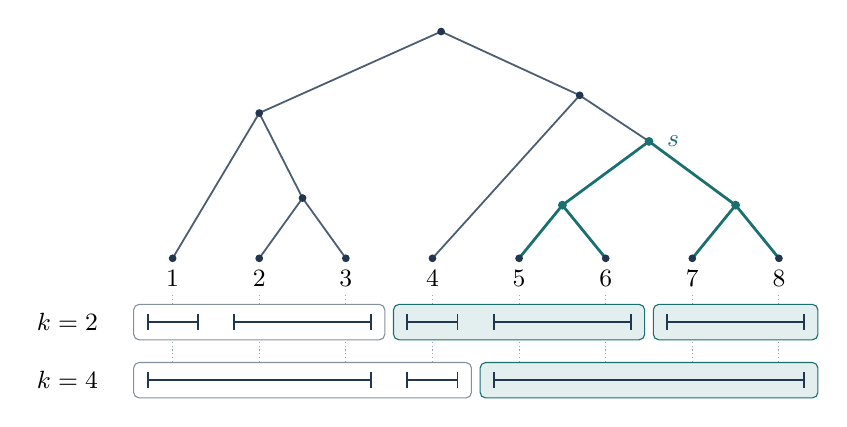
\begin{tikzpicture}[x=11mm,y=9mm,font=\small,
  branch/.style={draw=ink!80,line width=.65pt},
  marked/.style={draw=sea,line width=1pt},
  cluster/.style={draw=ink!55,rounded corners=2pt,fill=white},
  meets/.style={draw=sea,rounded corners=2pt,fill=sea!12},
  block/.style={|-|,draw=ink,line width=.7pt}]
\foreach \i in {1,...,8}
  \coordinate (leaf\i) at (\i,0);
\coordinate (root) at (4.1,3.2);
\coordinate (left) at (2,2.05);
\coordinate (right) at (5.7,2.3);
\coordinate (leftpair) at (2.5,.85);
\coordinate (s) at (6.5,1.65);
\coordinate (pairfive) at (5.5,.75);
\coordinate (pairseven) at (7.5,.75);
\draw[branch] (left)--(root)--(right)
              (leaf1)--(left)--(leftpair)
              (leaf2)--(leftpair)--(leaf3)
              (leaf4)--(right)--(s);
\draw[marked] (pairfive)--(s)--(pairseven)
              (leaf5)--(pairfive)--(leaf6)
              (leaf7)--(pairseven)--(leaf8);
\foreach \n in {root,left,right,leftpair} \fill[ink] (\n) circle (1.4pt);
\foreach \n in {s,pairfive,pairseven} \fill[sea] (\n) circle (1.6pt);
\node[right=3pt,text=sea] at (s) {$s$};
\foreach \i in {1,...,8} {
  \fill[ink] (leaf\i) circle (1.4pt);
  \node[below=1pt] at (leaf\i) {\(\i\)};
  \draw[densely dotted,ink!45] (\i,-.52)--(\i,-1.92);
}
\foreach \k/\y in {2/-.9,4/-1.72}
  \node[anchor=east] at (.25,\y) {\(k=\k\)};
\draw[cluster] (.55,-.65) rectangle (3.45,-1.15);
\foreach \l/\r in {4/6,7/8}
  \draw[meets] (\l-.45,-.65) rectangle (\r+.45,-1.15);
\draw[cluster] (.55,-1.47) rectangle (4.45,-1.97);
\draw[meets] (4.55,-1.47) rectangle (8.45,-1.97);
\foreach \l/\r in {1/1,2/3,4/4,5/6,7/8}
  \draw[block] (\l-.30,-.9)--(\r+.30,-.9);
\foreach \l/\r in {1/3,4/4,5/8}
  \draw[block] (\l-.30,-1.72)--(\r+.30,-1.72);
\end{tikzpicture}
\caption{An ordered tree of formula splits, with slots numbered in leaf
order. The bars show the maximal subtrees of at most \(k\) leaves, and
the boxes group consecutive bars into clusters. The highlighted subtree
has \(B_s=\{5,6,7,8\}\). It meets two clusters when \(k=2\) and lies in
one when \(k=4\), as the shaded boxes show. All four leaves therefore
receive the same displacement at the larger scale.}
\label{fig:cluster}
\end{figure}


Write $C_k(v)$ for the cluster of $v$. Displace every member of a
cluster in the same unit direction $a_C/\|a_C\|$ with weight $k/d$.
The combined displacement is
\[
            z_v=\sum_k\frac{k}{d}\frac{a_{C_k(v)}}{\|a_{C_k(v)}\|}.
\]
The weights sum to at most one. At a given scale, the inner products
within a cluster sum to $(k/d)\|a_C\|$. Thus
\[
       \sum_v\langle a_v,z_v\rangle
         =\sum_k\frac{k}{d}\sum_{C\text{ at scale }k}\|a_C\|
         \ge \tfrac12\lfloor\log d\rfloor .
\]

For the width bound, fix a node $s$ with $b=|B_s|$. At each scale
$k\ge b$ its entire subtree belongs to a single maximal block. Its
displacement at that scale is a common translation, which leaves its
width unchanged. At a scale $k<b$, the interval $B_s$ meets at most
$2+b/k$ clusters. All except possibly the two end clusters lie wholly
in the interval and have at least $k$ leaves. There are therefore at
most $2+b/k$ unit displacement directions on $B_s$ at this scale.

The set of combined displacements on $B_s$ is contained, up to
translation, in the Minkowski sum of these sets of directions scaled
by $k/d$. In the Gaussian formula, taking a maximum of a linear
functional gives monotonicity under inclusion and additivity on
Minkowski sums. Applying Equation~\eqref{eq:width-ball} to each set
of unit directions gives
\[
       \delta(\{z_v:v\in B_s\})
          \le C\sum_{k<b}\frac{k}{d}\sqrt{\log(2+b/k)}
          \le C_0\,\frac{b}{d}.
\]
At the $j$th dyadic scale below $b$, the summand is at most a
constant times $(b/d)2^{-j}\sqrt{j+2}$, whose sum converges.
\end{proof}

\subsection{From depth to size}

\begin{proof}[Proof of Theorem~\ref{thm:full-flat-graph}]
Let $e=d-1$ be the number of edges of $G$. Its split coefficient
tensor has terminal price $2ew$. Take a formula of depth $h$, and one
summand in Lemma~\ref{lem:formula-splits}. For this summand choose
the vectors $z_v$ of Lemma~\ref{lem:formula-placement} and perform the
map at slot $v$ at the site $\lambda z_v$, with $\lambda\ge0$.
Share each address among its descendants at those sites, then send the
$\deg(v)$ output indices of each slot to their terminals by $q$-state
wires. The resulting upper bound on the terminal price is
\begin{equation}\label{eq:full-flat-profile}
 \begin{aligned}
   2ew
     &-w\lambda\sum_v\langle a_v,z_v\rangle
      +\tfrac12 w\lambda^2\sum_v\deg(v)\|z_v\|^2\\
     &+\lambda\sum_s\ell_s\,\delta(\{z_v:v\in B_s\}).
 \end{aligned}
\end{equation}
The first line uses Equation~\eqref{eq:move} for the output wires.
The second is the exact price of the independent address labels.
Its coefficient of $\lambda$ is at most $C_0h$, since
\[
        \sum_s\ell_s\frac{|B_s|}{d}
            =\frac1d\sum_v\sum_{s:\,v\in B_s}\ell_s\le h .
\]
The first-order shortening in the first line is at least
$c_0w\lambda\log d$, and the quadratic term is at most $ew\lambda^2$.
If $h\le c_1w\log d$ for sufficiently small $c_1$, choosing
$\lambda=c_2(\log d)/d$ with $c_2>0$ sufficiently small bounds
the price of each summand by
\[
                  2ew-c_3\,\frac{w(\log d)^2}{d}
\]
for an absolute $c_3>0$.

All summands now have the same $2e$ terminal sites. By
Equations~\eqref{eq:ordinary} and~\eqref{eq:width-ball}, adding the
summands of Lemma~\ref{lem:formula-splits} costs a premium of at most
\[
                O\bigl(d\sqrt{\log(2d)}\,\log(d(h+2))\bigr).
\]
The ratio of this premium to the saving is $O(w^{-1/3}\log w)$,
uniformly for $2\le d\le w^{1/3}$ and $h\le c_1w\log d$. Thus the
coefficient tensors of all such formulas lie in a fixed price
sublevel strictly below $2ew$ for all sufficiently large $w$.
The sublevel is Zariski closed, and extraction of one variable per
slot is a linear map on degree-$d$ components. The graph polynomial
is therefore excluded even from the degree-component border of the
depth-$h$ formulas. Unfolding a binary circuit into a formula
preserves its depth and its output, giving the claimed circuit depth
bound as well.

Finally, a formula of size $m$ can be balanced to depth
$O(\log(m+2))$ over every field~\cite{Brent}. For the division-free
construction, push subtraction signs to the affine leaves and select
a subformula $g$ containing between a third and two thirds of the
leaves. The output equals $ag+b$, where $a$ is the product of the
siblings at the multiplication gates on the path from $g$ to the
root, and $b$ is the original expression evaluated with $g=0$.
Each of $a,b,g$ uses at most two thirds of the original leaves plus
one. Recursion down to constant size gives the desired depth.
Balancing preserves the polynomial before closure, so the depth
bound yields the degree-component border formula size in the theorem.
\end{proof}

For a path, Theorem~\ref{thm:full-flat-graph} and the bisection formula
give matching exponents. The estimate extends to
$2\le d\le(\log q)^B$ for any fixed $B>1/3$, with lower bound
$q^{\Omega_B(\log d)}$ on every tree in this range. When
$d>(\log q)^{1/3}$, project to a subtree on
$\lfloor(\log q)^{1/3}\rfloor$ vertices. The logarithm of this
subtree size is $\Omega_B(\log d)$, and the quadratic cost of the
border formula projection in Lemma~\ref{lem:projection} only changes
the implied constant in the exponent.

Taking $q=n$ and projecting the $n$-vertex path to its first
$\lfloor(\log n)^{1/3}\rfloor$ vertices gives degree-component
border formula size $n^{\Omega(\log\log n)}$. Its layered ABP has
polynomial size, so this proves the path separation in
Theorem~\ref{thm:main}.

The same lower bound transfers to the order-$n$ determinant. Take
$q=\lfloor\sqrt n\rfloor$ and $d=\lfloor(\log q)^{1/3}\rfloor$.
Let $A$ be the weighted adjacency matrix of the layered ABP in
topological order. It is strictly upper triangular, so
$\det(I-A)=1$. The source--sink entry of
$(I-A)^{-1}=\sum_{j\ge0}A^j$ is the path polynomial. By the
cofactor formula it is also a signed minor of $I-A$ of order
$(d-1)q+1\le n$~\cite{Valiant,MalodPortier}. Absorb the sign into
one row and pad with an identity block to obtain an affine projection
of the order-$n$ determinant. Lemma~\ref{lem:projection} transfers
the short-path lower bound and completes the proof of
Theorem~\ref{thm:main}.

\section{Classification of graph state sums}\label{sec:graph-classification}

The three separation witnesses also determine which graph families
admit polynomial-size computations of their state sums. Recall that
\(Z_{G,q}\) assigns a separate variable to every choice of the
\(q\)-valued labels on the
edges incident to each vertex, as in Equation~\eqref{eq:graph}.
We measure size in terms of the number \(d\) of vertices and the
alphabet size \(q\). A single vertex of degree \(t\) thus supplies
\(q^t\) distinct input variables. In a multigraph every parallel edge
carries its own label and counts separately towards degrees and cuts.

Write \(m(G)\) for the largest order of a connected component and
\(\Delta(G)\) for the maximum degree. The \emph{cutwidth}
\(\operatorname{cw}(G)\) is the minimum, over vertex orders, of the
largest number of edges crossing from a prefix to its complement.
A \emph{tree decomposition} consists of a tree of vertex sets, called
bags. The bags containing a given vertex form a nonempty connected
subtree, and the two ends of each edge belong to a common bag. The
\emph{treewidth} \(\operatorname{tw}(G)\) is the minimum largest bag
size minus one. Requiring the decomposition tree to be a path gives
\emph{pathwidth}, denoted by \(\operatorname{pw}(G)\).

\begin{theorem}[Polynomial-size graph state sums]\label{thm:graph-classification}
Fix a field and a class \(\mathcal G\) of nonempty finite loopless
multigraphs. In each model below, a single polynomial in \(d+q\)
bounds the size of \(Z_{G,q}\) for every \(G\in\mathcal G\) and
every integer \(q\ge2\) if and only if the indicated parameters
are bounded on \(\mathcal G\).
\begin{center}
\begin{tabular}{@{}ll@{}}
\toprule
\textup{Arithmetic model} & \textup{Bounded graph parameters}\\
\midrule
Formula & \(m(G)\) and \(\Delta(G)\)\\
Algebraic branching program & \(\operatorname{cw}(G)\)\\
Circuit & \(\operatorname{tw}(G)\) and \(\Delta(G)\)\\
\bottomrule
\end{tabular}
\end{center}
For a sequence \(G_n\) with \(|V(G_n)|\le n^{O(1)}\), the same criteria,
uniformly in \(n\), characterize polynomial size for \(Z_{G_n,n}\).
In both formulations the upper bounds hold for exact computation, and
the necessary conditions already hold for degree-component border size.
\end{theorem}

\subsection{The degree obstruction}

Two vertices joined by \(t\) parallel edges give a dot product of two
tables of length \(q^t\). This graph has component order two and
treewidth one for every \(t\). The coefficient matrix of the dot
product is the \(q^t\)-by-\(q^t\) identity. The same obstruction occurs
at any vertex \(v\) of degree \(t\). Flatten the coefficient tensor
across the slot at \(v\) and all remaining slots. Each of its \(q^t\)
rows has nonempty support, since every choice of incident labels
extends to a full edge labeling. The supports are disjoint, since the
table indices at the neighbors determine all these labels. The rank is
therefore \(q^t\) over every field.

This rank bound still detects large tables when affine input forms
are free. For a size-\(s\) computation, let \(U\) be the span of the
linear parts of its affine inputs in the variables at \(v\). There are
\(O(s+1)\) such inputs in each of the three models. In the part of the
output linear in those variables, each product of input forms takes
its \(v\)-linear term from exactly one factor. Extracting a coefficient
in the other slots therefore gives a vector in \(U\). The flattening
has rank at most \(\dim U=O(s+1)\). Since this condition is defined
by vanishing minors of the slot tensor, it holds also on the
degree-component closure.

Consequently a polynomial size bound requires bounded degree. For a
graph class take \(q\ge\max\{2,d\}\) arbitrarily large for each \(G\).
For a sequence take \(q=n\). In both cases the bound
\(q^{\Delta(G)}=O(s+1)\) forces a uniform bound on \(\Delta(G)\).
In the branching-program row, cutwidth already controls degree. In
any order the edges incident to \(v\) cross either the cut immediately
before \(v\) or the cut immediately after it, so
\(\Delta(G)\le2\operatorname{cw}(G)\).

\subsection{Exact computations from graph decompositions}

\paragraph{Formulas.}
The state sum factors over connected components. In a component on
at most \(a\) vertices, enumerate its at most \(q^{\Delta(G)a/2}\)
edge labelings. Each labeling contributes one product of local table
entries. Summing these products within each component and multiplying
the results gives a formula of size \(O((d+1)q^{\Delta(G)a/2})\).
An isolated vertex contributes its single variable.

\paragraph{Branching programs.}
Take an order of cutwidth \(k\), and place one layer after each
prefix. A state records the labels of the at most \(k\) edges that
cross the current cut. At the next vertex, the state gives the labels
on its backward edges. Choose labels for its forward edges, read the
resulting table entry as the transition weight, and retain just the
labels that cross the next cut. Every full edge labeling determines
one source--sink path of the required weight, and every such path
comes from a labeling. There are at most \(dq^{k+\Delta(G)}\)
transitions.

\paragraph{Circuits.}
A tree decomposition of width \(k\) yields a circuit of size
\(O((d+1)q^{\Delta(G)(k+1)})\). Contract adjacent bags whenever one
contains the other, keeping the larger bag, and root the remaining
tree. Each nonroot bag contains a vertex absent from its parent.
By connectedness this is the highest occurrence of that vertex,
so the decomposition has at most \(d+1\) bags.

Assign each vertex table to a bag containing the vertex. Replace
the vertex set of each bag by the list of all edges incident to that
set. The new list has at most \(\Delta(G)(k+1)\) entries and includes
every edge label needed by a table assigned there. For each edge,
the bags containing it still form a connected subtree, since the
subtrees of its endpoints intersect. This construction is related to
the characterization of edge contraction complexity by line-graph
treewidth due to Markov and Shi~\cite{MarkovShi}.

Compute a table at each bag, starting at the leaves. For each assignment
on its edge list, multiply the local vertex entries by the child
tables evaluated on the edges common to the child and the bag. Sum
these values over the labels absent from the parent. The resulting
table is indexed by the labels shared with the parent. Connectedness
ensures that every label used on both sides of this boundary occurs
in the intersection, and that each other label is summed out exactly
once. At the root the output is \(Z_{G,q}\). The total number of
child factors and assigned vertex tables over all bags is \(O(d+1)\),
giving the stated gate count.

\subsection{Transferring lower bounds through graph minors}

To use a graph minor \(H\), we must convert a computation for its
host \(G\) into one for \(Z_{H,q}\). Each vertex of \(H\) is represented
by a connected set of host vertices. The construction routes the labels
entering this set to a single vertex, where its table entry is read.
The required host alphabet depends only on the degree of \(H\).

\begin{lemma}[Projection to a minor]\label{lem:graph-minor}
Let \(H\) be a loopless minor of a finite loopless multigraph \(G\),
and set \(b=\max\{1,\lfloor\Delta(H)/2\rfloor\}\).
If \(q^b\le n\), then \(Z_{H,q}\) is a projection of \(Z_{G,n}\)
using only variables, zero and one.
\end{lemma}

\begin{proof}
Choose disjoint connected branch sets for the vertices of \(H\).
For each edge of \(H\), choose a distinct host edge joining its two
branch sets. Use the first \(q\) states on each chosen edge to carry
its label. Within the branch set for a vertex \(v\), choose a spanning
tree and weight each tree vertex by the number of chosen edges meeting
it. The total weight is \(\deg_H(v)\). Root the tree at a weighted
centroid, so every component below the root has at most half the total
weight. To find such a root, move into any neighboring component of
weight greater than half. Each move leaves less than half the weight
behind, so this walk on a finite tree terminates.

Fix an ordering of the chosen edges. On each tree edge from a child
to its parent, encode in one host state the tuple of labels entering
the child's subtree, in the induced order. The tuple has at most
\(\lfloor\deg_H(v)/2\rfloor\) entries, so \(q^b\le n\) makes all its
values available. At a nonroot vertex, set a local entry to one
precisely when the tuple sent to its parent agrees with the tuples
from its children and the labels of the chosen edges meeting the
vertex. At the root these same data specify the entire tuple at \(v\).
Use the corresponding variable of \(Z_{H,q}\) there. This also covers
an isolated vertex of \(H\), whose tuple is empty.

Pin all unused edges to a single state and give unused vertices
weight one on legal inputs. Set inconsistent table entries and unused
encodings to zero. Each labeling of \(H\) extends uniquely to a
surviving host labeling, because every tuple on a tree edge is forced
by the chosen external labels. The corresponding monomial is exactly
the product of the variables read at the roots.
\end{proof}

\begin{proof}[Necessity in Theorem~\ref{thm:graph-classification}]
First consider a sequence \(G_n\) of polynomially bounded order.
The degree obstruction allows us to assume \(\Delta(G_n)\) bounded.
Each of the remaining unbounded parameters forces its own witnesses.

\begin{itemize}
\item If component order is unbounded, arbitrarily long paths occur
as subgraphs. In a graph of bounded degree, balls of any fixed radius
have bounded order.
\item If cutwidth is unbounded, so is pathwidth. Indeed
\[
 \operatorname{pw}(G)\le\operatorname{cw}(G)
 \le\Delta(G)(\operatorname{pw}(G)+1).
\]
For the first inequality, form each path bag from the next vertex in
an order and the processed vertices with an edge to an unprocessed
vertex. For the second, order the vertices by their first occurrence
in a path decomposition. At each cut, every processed vertex with a
future neighbor belongs to the bag in which the next vertex first
occurs. The crossing edges are therefore incident to at most
\(\operatorname{pw}(G)+1\) processed vertices. The excluded-forest
theorem gives complete binary trees of arbitrarily many levels as
minors~\cite{BRST}.
\item If treewidth is unbounded, square grids of arbitrarily large side
length occur as minors by the excluded-grid theorem
\cite{RSgrid,ChekuriChuzhoy}.
\end{itemize}

Treewidth and pathwidth depend only on the underlying simple graph.
The tree and grid minors just obtained are thus also minors of the
original multigraphs. For every fixed witness size, the corresponding
minor occurs along a subsequence with \(n\to\infty\).
Lemma~\ref{lem:graph-minor} retains \(q=n\) for paths and binary trees
and permits \(q=\lfloor\sqrt n\rfloor\) for grids.

Suppose the host border size were polynomial in \(n\).
Lemma~\ref{lem:projection}, applied with host degree \(|V(G_n)|\),
would give an upper bound \(n^C\) for all projected witnesses, with
\(C\) independent of the witness size. But the short-witness lower
bounds grow as \(q^{\Omega(\log d')}\) for formulas on a path of
\(d'\) vertices, \(q^{\Omega(\sqrt h)}\) for ABPs on a binary tree of
\(h\) levels, and \(q^{\Omega(\sqrt r)}\) for circuits on an
\(r\)-by-\(r\) grid (Theorems~\ref{thm:full-flat-graph},
\ref{thm:b} and~\ref{thm:grid}). Choose the witness size large enough
that its exponent in \(n\) exceeds \(C\), even accounting for the
square root in the grid alphabet. Then take \(n\) sufficiently large
along the corresponding subsequence so that the hypotheses of the
short-witness bound hold. This proves necessity for sequences.

Finally, if a graph class has an unbounded parameter in its row, choose
graphs on which that parameter tends to infinity. Give each graph a
distinct index \(n\) at least its order and fill the other indices from
one fixed graph in the class. A uniform polynomial bound in \(d+q\)
would give a polynomial bound in \(n\) for this sequence at \(q=n\),
contrary to the preceding argument.
\end{proof}


\bibliographystyle{plainnat}
\bookmarksetup{startatroot}
\bibliography{references}
\end{document}
